% ============================================================================
% ISMSIT 2026 -- position paper derivado de docs/artigo_final/main.tex
%
% Versao ANONIMIZADA para a revisao duplo-cega exigida pela conferencia.
% Para a versao camera-ready, trocar o bloco \author ativo pelo bloco
% comentado logo abaixo dele.
%
% Compilacao: pdflatex -> bibtex -> pdflatex -> pdflatex
% ============================================================================
\documentclass[conference]{IEEEtran}
\usepackage[utf8]{inputenc}
\usepackage[T1]{fontenc}
\usepackage[english]{babel}
\usepackage{cite}
\usepackage{graphicx}
\usepackage{textcomp}
\usepackage{booktabs}
\usepackage{array}
\usepackage{tabularx}

\title{Moderating Before Publication: A Position on LLM-Assisted
Prospective Moderation of Unproductive Debates}

\author{\IEEEauthorblockN{Anonymous Author(s)}
\IEEEauthorblockA{\textit{Affiliation omitted for double-blind review}}}

% --- Camera-ready (restaurar apos o aceite) ---------------------------------
% \author{\IEEEauthorblockN{Guilherme Moura}
% \IEEEauthorblockA{\textit{Systems Engineering and Computer Science} \\
%       \textit{Program (PESC/COPPE)} \\
%       \textit{Federal University of Rio de Janeiro} \\
%       Rio de Janeiro, Brazil \\
%       gpcmoura@cos.ufrj.br}
% \and
% \IEEEauthorblockN{Luiz Filipe Brandi}
% \IEEEauthorblockA{\textit{Systems Engineering and Computer Science} \\
%       \textit{Program (PESC/COPPE)} \\
%       \textit{Federal University of Rio de Janeiro} \\
%       Rio de Janeiro, Brazil \\
%       brandi@cos.ufrj.br}
% \and
% \IEEEauthorblockN{Ramon Chaves}
% \IEEEauthorblockA{\textit{Systems Engineering and Computer Science} \\
%       \textit{Program (PESC/COPPE)} \\
%       \textit{Federal University of Rio de Janeiro} \\
%       Rio de Janeiro, Brazil \\
%       ramonchaves@cos.ufrj.br}
% \and
% \IEEEauthorblockN{Daniel Schneider}
% \IEEEauthorblockA{\textit{Systems Engineering and Computer Science} \\
%       \textit{Program (PESC/COPPE)} \\
%       \textit{Federal University of Rio de Janeiro} \\
%       Rio de Janeiro, Brazil \\
%       schneider@cos.ufrj.br}
% }
% ----------------------------------------------------------------------------

\begin{document}

\maketitle

\begin{abstract}
Moderation on digital platforms operates predominantly after publication,
removing, flagging, or sanctioning content when much of the harm has already
been done. Prior work proposed a five-dimension sociotechnical model for
mitigating unproductive debates, in which one dimension regulates conduct
before a message is posted by offering reformulations of hostile candidate
messages. This position paper argues that evaluating such prospective
moderation raises a problem that is conceptual before it is empirical: once a
candidate message is rewritten, it ceases to exist as observable data, and so
does the course the debate would have taken from it. Drawing on Angenot's
account of the dialogue of the deaf and on the literature that distinguishes
impoliteness, incivility, and intolerance, the paper contends that prospective
moderation should act on the form of an exchange rather than on its content,
and that it should intervene where hostility shifts from the argument to the
person. It then discusses simulation with polarized agents based on large
language models as a lens that makes the candidate and the published message
observable at the same time, and it makes explicit what such a lens cannot
capture: author agency, perceived hostility, and the behavior of real users.
Open questions are raised for a research agenda on the composition of
mitigation mechanisms.
\end{abstract}

\begin{IEEEkeywords}
unproductive debates, prospective moderation, LLM agents, online incivility,
synthetic personas, simulation
\end{IEEEkeywords}

\section{Introduction}\label{sec:intro}

The quality of digital public debate is undermined by dynamics that stem
neither from the ignorance nor from the bad faith of its participants. Part of
the problem is inherent to dialogue itself: Angenot argued that mutual
incomprehension is a structural condition of social life, which he described
as a \textit{dialogue of the deaf}~\cite{angenot2008dialogues}. Platform
architecture amplifies this condition. Oriented toward metric-driven
engagement, platforms reward impulsive reaction over argumentative
elaboration, while the moderation mechanisms at their disposal operate
predominantly in a reactive way, removing, flagging, or sanctioning content
after publication, when the harm of what was published has often already been
done.

Prior work characterized this phenomenon as \textit{unproductive debate} and
proposed a conceptual model for its mitigation, in which Generative AI acts as
a transversal mediator, guided by the principle of human--AI
symbiosis~\cite{moura2026hostility}. The model distributes mitigation over
five dimensions. The first four act on the exchange itself: Interactional
Deceleration (D1) slows the rhythm at which replies follow one another;
Argumentative Structuring (D2) organizes and displays the arguments in play;
Collaborative Curation (D3) keeps the evidence behind claims traceable and on
record; and Mediated Exposure to Divergent Perspectives (D4) calibrates how
much of the opposing side reaches each participant. The fifth, Participatory
Moderation (D5), holds a distinctive position: rather than acting on the
exchange, it regulates the \textit{conduct} of those who take part in it, and
it does so in two modes: proactively, by configuring the discursive space
before conflict sets in, and reactively, by containing escalation while a
debate is still under way. In the reactive mode, the intervention can take
place before a message is published, in the interval between its production
and its posting; this pre-publication intervention is what this paper calls
\textit{prospective moderation}.

This location, between production and posting, is precisely what makes the
intervention difficult to evaluate in real environments. Observing the effect of a reformulation would require
access to the message that was not published. On a real platform, a candidate
message that is withdrawn or rewritten simply ceases to exist as observable
data, and so does whatever would have followed from it in the debate.

This paper takes the position that this observability problem must be
confronted before any claim about the effectiveness of prospective moderation
can be made, and that simulation with agents based on Large Language Models
(LLMs) offers a lens complementary to field studies: by instantiating
polarized artificial debaters and recording each message before and after the
intervention, it renders observable what a platform necessarily hides. No
experiment is reported here. The positions derive from an ongoing research
program that examines D5 empirically, whose protocol and findings will be
reported separately; the aim of this paper is to make explicit the conceptual
choices that such an evaluation requires and the limits it cannot overcome.
Specifically, the paper makes the following contributions:

\begin{itemize}
\item \textbf{Form over content.} Building on the three pathologies of
unproductive debate described by Angenot, it argues that prospective
moderation should act on the form in which premises are published, not on
their content.
\item \textbf{A principled threshold.} Drawing on the incivility literature,
it argues that intervention belongs where hostility migrates from the argument
to the person, and that hostility is better treated as an ordinal severity
than as a binary label or a probability of perceived toxicity.
\item \textbf{Simulation as a lens.} It discusses simulation with LLM agents
as a means of observing the unpublished message, the conditions under which
such simulation is informative, and the questions it leaves open.
\end{itemize}

The remainder of the paper is organized as follows.
Section~\ref{sec:related} reviews related work. Section~\ref{sec:foundations}
discusses unproductive debate and the place of prospective moderation.
Section~\ref{sec:lens} examines simulation as a lens on the unpublished
message. Section~\ref{sec:open} raises open questions, and
Section~\ref{sec:conclusion} concludes.

\section{Related Work}\label{sec:related}

\subsection{Incivility and Its Measurement}\label{sec:incivility}

Political communication research distinguishes phenomena that are often
conflated. Papacharissi~\cite{papacharissi2004democracy} defines
\textit{impoliteness} as the violation of interpersonal norms of etiquette,
such as a rude tone or vulgar language, and \textit{incivility} as behavior
that threatens democratic values through the delegitimization and exclusion of
the interlocutor: being rude is not the same as violating democratic norms.
Coe, Kenski, and Rains~\cite{coe2014online} operationalized incivility into
five binary types (name-calling, aspersion, lying, vulgarity, and pejorative
for speech), a taxonomy later applied to the study of intergroup
factors~\cite{rains2017incivility}. The public, however, perceives these types
as differing in severity~\cite{kenski2020perceptions}, which suggests a latent
ordinal dimension that a categorical taxonomy does not express.

Rossini~\cite{rossini2022beyond} advanced Papacharissi's distinction by
separating incivility from \textit{intolerance}: the former tends to occur in
discursively engaged exchanges, with justified opinions and genuine
confrontation of disagreement, whereas the latter appears in homogeneous
discussions with less deliberation. The implication is counterintuitive:
interpersonal incivility is not incompatible with democratic discussion, and
what threatens deliberation is intolerance. Bentivegna and
Rega~\cite{bentivegna2022searching} decomposed the phenomenon into
impoliteness, individual delegitimization, which frames the opponent as
irrational, dishonest, or morally deficient for who they are, and
institutional delegitimization. Mutz and Reeves~\cite{mutz2005new} offered
empirical evidence that hostility can be isolated from content: by
manipulating the incivility of televised debates while holding their content
constant, they showed that lower hostility preserves political trust, a condition for productive political debate. The
position taken in this paper carries that premise over to digital platforms,
where mitigating hostility is a condition for healthier and more productive
debates.

As for measurement, continuous probabilistic scores, such as those provided by
commercial toxicity detection services, estimate the probability that a
reader will perceive a text as toxic, which is a quantity distinct from
severity. Kennedy et al.~\cite{kennedy2020constructing} proposed a more
rigorous alternative, decomposing the construct into ordinal components rated
by crowd workers and transforming them into a variable with interval
properties.

\subsection{Pre-Publication Interventions and LLM Agents}\label{sec:interventions}

A body of work examines interventions that act before publication, which is
precisely where D5 operates. Argyle et al.~\cite{argyle2023leveraging} showed
in a field experiment that rephrasing suggestions generated by an LLM improve
the perceived quality of polarized political conversations without
manipulating the participants, who could accept, edit, or ignore each
suggestion. Katsaros, Yang, and Fratamico~\cite{katsaros2022reconsidering}
reported that intervening during message creation decreased offensive content
on Twitter, and Tessler et al.~\cite{tessler2024ai} showed that AI mediation
can help human groups find common ground in democratic deliberation. Brandi et
al.~\cite{brandi2026nudge}, in turn, proposed an LLM-mediated framework for
nudge-based text detoxification that reframes the proactive mitigation of hate
speech as assisted decision-making, with the system acting as a cognitive
mediator: rather than rewriting the text automatically, it presents less
toxic alternatives, including non-coercive default options, while keeping the
original version accessible, in order to avoid user passivity and the
perception of algorithmic censorship. In all these approaches, the author
retains the final decision on what is published, and the acceptance rate is
itself a central outcome. Katsaros et al.\
observed, for instance, that 69\% of the flagged messages were posted without
revision~\cite{katsaros2022reconsidering}, so the decision of users directly
shapes the measured effect.

Simulations with LLM agents raise a different concern. Chuang et
al.~\cite{chuang2023simulating} simulated opinion dynamics with networks of
LLM-based agents and documented a bias that is critical for any simulation of
conflict: such agents tend toward consensus and politeness. Structured
datasets of synthetic personas, such as a recent collection of about one
million personas described along 1,290 categorical
dimensions~\cite{li2026matraix}, in turn make it possible to compose groups of
antagonistic debaters through explicit classification rules, in a
reproducible and traceable way.

\section{Unproductive Debate and Prospective Moderation}\label{sec:foundations}

\subsection{The Dialogue of the Deaf}\label{sec:angenot}

Angenot argues that mutual incomprehension in debate derives neither from
logical failure nor from flaws of character, but from a structural condition
of social life~\cite{angenot2008dialogues}. Three analytical categories follow
from this thesis~\cite{angenot2008dialogues,angenot2010discurso}:

\begin{itemize}
\item \textbf{Discursive incommensurability.} Interlocutors do not share
worldviews, values, or presuppositions about what counts as truth; they
operate in entirely distinct discursive universes.
\item \textbf{Rhetoric of incomprehension.} The adversary is recognized not as
a rational being but as irrational or degenerate, and is delegitimized for
what they think, usually through irony, stereotypes, and caricature.
\item \textbf{Illusion of rationality.} Participants expect the debate to
converge on consensus when, in fact, they defend their views in order to win
or to reaffirm their own convictions.
\end{itemize}

The thesis carries a design consequence. If incomprehension were an
informational deficit, mitigation would consist of supplying the missing
information; if it were a logical failure, of correcting the reasoning. Being
structural, it is reached by neither strategy. What remains within reach is
the form of the interaction: reformulating how each premise is published
without eroding the content under dispute. This is the first position
defended here: prospective moderation should act on form, not on content. The
evidence that hostility can vary while content is held
constant~\cite{mutz2005new} suggests that the separation is feasible.

The categories describe a mechanism rather than an intensity. A severity
measure indicates how much hostility a message carries; the pathologies
indicate which dynamics of the dialogue of the deaf are at work. Messages of
very different severity may exhibit the same pathology, and a single message
may exhibit more than one, so severity and mechanism call for separate
records. Angenot's work is established in the traditions of rhetoric and
discourse analysis, but the operationalization of his categories as signals
for computational detection by LLM agents has no direct precedent in the
literature, which also means that there is no external benchmark against
which to validate it.

\subsection{Prospective Moderation in the Five-Dimension Model}\label{sec:d5}

The predecessor model~\cite{moura2026hostility} grounds the five dimensions
introduced in Section~\ref{sec:intro} in a knowledge-creation spiral. D1 to D4
each support one phase of that spiral, slowing the exchange, structuring it,
qualifying its evidence, and dosing contact with opposing views. D5
corresponds to no isolated phase: by regulating conduct instead of qualifying
content, it provides the governance infrastructure without which the other
four dimensions cannot remain operative. The model does not, however, treat D5
as sufficient on its own, since it expects mitigation from the combination of
the five dimensions, a point to which Section~\ref{sec:conclusion} returns. In
the model, the AI layer acts as a sociotechnical mediator that summarizes
histories, detects violations of norms, and offers reformulations, the last of
which is the function at stake here. Since the moderation cycle considered in
this paper does not yet involve human participation, this pre-publication
facet of D5 is called \textit{prospective} rather than participatory
moderation.

\subsection{What to Moderate: From the Argument to the Person}\label{sec:threshold}

If rudeness does not amount to a violation of democratic
norms~\cite{papacharissi2004democracy} and incivility can coexist with
productive deliberation~\cite{rossini2022beyond}, a moderator that intervenes
on every sharp message would treat legitimate disagreement as a problem to be
corrected. The second position defended here is that the intervention
threshold should operationalize the conceptual boundary between impoliteness
and incivility~\cite{papacharissi2004democracy,rossini2022beyond}, that is,
the point at which the target of hostility migrates from the argument to the
person. Short of that boundary, harshness and sarcasm aimed at an argument
remain part of a debate that may be unproductive but is legitimate; beyond
it, the opponent, rather than the position, becomes the object of the
message.

Locating such a boundary requires a measure capable of expressing it. Binary
classification restricts the information available about
severity~\cite{kennedy2020constructing}, and probabilistic toxicity scores
answer a different question. Hostility is therefore better treated as an
ordinal severity with discrete levels, for three reasons: instructing an LLM
requires categories with verbal descriptors; comparing the judgment of the
instrument that moderates with that of the instrument that evaluates requires
a common scale; and the qualitative analysis of moderation records requires
levels that can be named. Such a scale need not adopt an existing instrument,
since it can synthesize distinctions already consolidated in the literature
reviewed in Section~\ref{sec:incivility}.

Table~\ref{tab:rubric} illustrates such a synthesis. It orders five bands by
increasing severity. In the first two, hostility remains aimed at the
argument; from the third onward, it reaches the person, first indirectly,
through the caricature of a position, and then explicitly, through
delegitimization and personal attack. The boundary defended above therefore
falls between the second and third bands: impatience and sarcasm directed at
an argument are left untouched, whereas ridiculing the opponent's position
already marks the shift toward the person. The excerpts, all taken from
simulated debates on the same topic, show how each band appears in an actual
message. The operational descriptors given to the agents, and the scores they
produce, are left to the empirical report.

\begin{table*}[t]
\caption{An Illustrative Ordinal Rubric of Hostility, from the Argument to the Person}
\label{tab:rubric}
\centering
\renewcommand{\arraystretch}{1.2}
\begin{tabularx}{\textwidth}{@{}>{\raggedright\arraybackslash}p{1.95cm}>{\raggedright\arraybackslash}p{1.45cm}>{\raggedright\arraybackslash}X>{\raggedright\arraybackslash}p{3.6cm}>{\raggedright\arraybackslash}X@{}}
\toprule
\textbf{Band} & \textbf{Target} & \textbf{What characterizes it} & \textbf{Conceptual anchors} & \textbf{Excerpt from a simulated debate} \\
\midrule
No hostility & Argument & Disagreement in a neutral or respectful tone; the message engages the opposing argument & Disagreement distinct from incivility~\cite{papacharissi2004democracy,rossini2022beyond} & ``Prohibition has created a black market fueled by violence and exploitation.'' \\
Harsh tone & Argument & Impatience, harshness, or sarcasm directed at the argument, with no delegitimization of the opponent & Impoliteness~\cite{papacharissi2004democracy}; aspersion~\cite{coe2014online} & ``You're probably here to spout some tired pro-legalization talking points, right?'' \\
\midrule
\multicolumn{5}{@{}l}{\textit{Boundary: the target of hostility migrates from the argument to the person}} \\
\midrule
Caricature & Person, indirectly & The opponent's position is reduced and ridiculed; contempt is coded rather than stated & Rhetoric of incomprehension~\cite{angenot2008dialogues}; pejorative for speech~\cite{coe2014online}; transition toward incivility~\cite{rossini2022beyond} & ``Newsflash: it's not about `personal freedom' or some hippie fantasy about `harm reduction.'\,'' \\
Delegitimization & Person & The opponent is framed as irrational, dishonest, or morally deficient; labels replace engagement & Individual delegitimization~\cite{bentivegna2022searching}; name-calling~\cite{coe2014online,kenski2020perceptions} & ``[\ldots] your `moral high ground' routine is just a thin veil for your own dogmatic thinking.'' \\
Personal attack & Person & Direct insult; language aimed at the opponent's dignity, identity, or worth & Intolerance~\cite{rossini2022beyond}; highest perceived incivility~\cite{kenski2020perceptions}; effects on political trust and productive debate~\cite{mutz2005new} & ``You're a waste of space, a blight on the face of humanity.'' \\
\bottomrule
\multicolumn{5}{@{}p{\textwidth}@{}}{\footnotesize Bands are ordered by increasing severity. Excerpts are verbatim fragments of messages published in debates on drug legalization simulated by the research program from which these positions derive; each was assigned to its band by an evaluator blind to the condition. They illustrate the bands and are not reported as findings.}
\end{tabularx}
\end{table*}

A caveat concerns the object of measurement. The hostility at stake is the
one manifested in the published text, as classified by an agent instructed
with an explicit rubric. It is neither the hostility perceived by human
readers nor the hostile intent of the author: these quantities appear close
but are distinct, and both lie beyond the reach of a design based on
artificial agents.

\section{The Unpublished Message: Simulation as a Lens}\label{sec:lens}

\subsection{Two Complementary Lenses}\label{sec:lenses}

Field studies of pre-publication
interventions~\cite{argyle2023leveraging,katsaros2022reconsidering} measure
effects on human participants on real platforms and therefore capture the
behavioral dimension that no simulation reaches. They cannot, however,
isolate the effect of the reformulation itself, because the rejected
candidate message does not enter the analysis. Simulation with LLM agents
makes the inverse move: it sets aside the behavioral criterion, namely the
author's decision about the reformulation, in order to gain full access to
what would have been published. By instantiating polarized artificial
debaters, recording each message before and after the intervention, and
submitting debates with and without moderation to an evaluator blind to the
condition, it becomes possible to estimate the effect of prospective
moderation under controlled conditions. Fig.~\ref{fig:pipeline} outlines this
conceptual pipeline, together with the conditions discussed in
Section~\ref{sec:conditions}. Table~\ref{tab:lenses} contrasts what each lens
makes observable. The two lenses are complementary rather than competing, and
neither of them, on its own, settles whether prospective moderation works.

\begin{figure*}[!t]
\centering
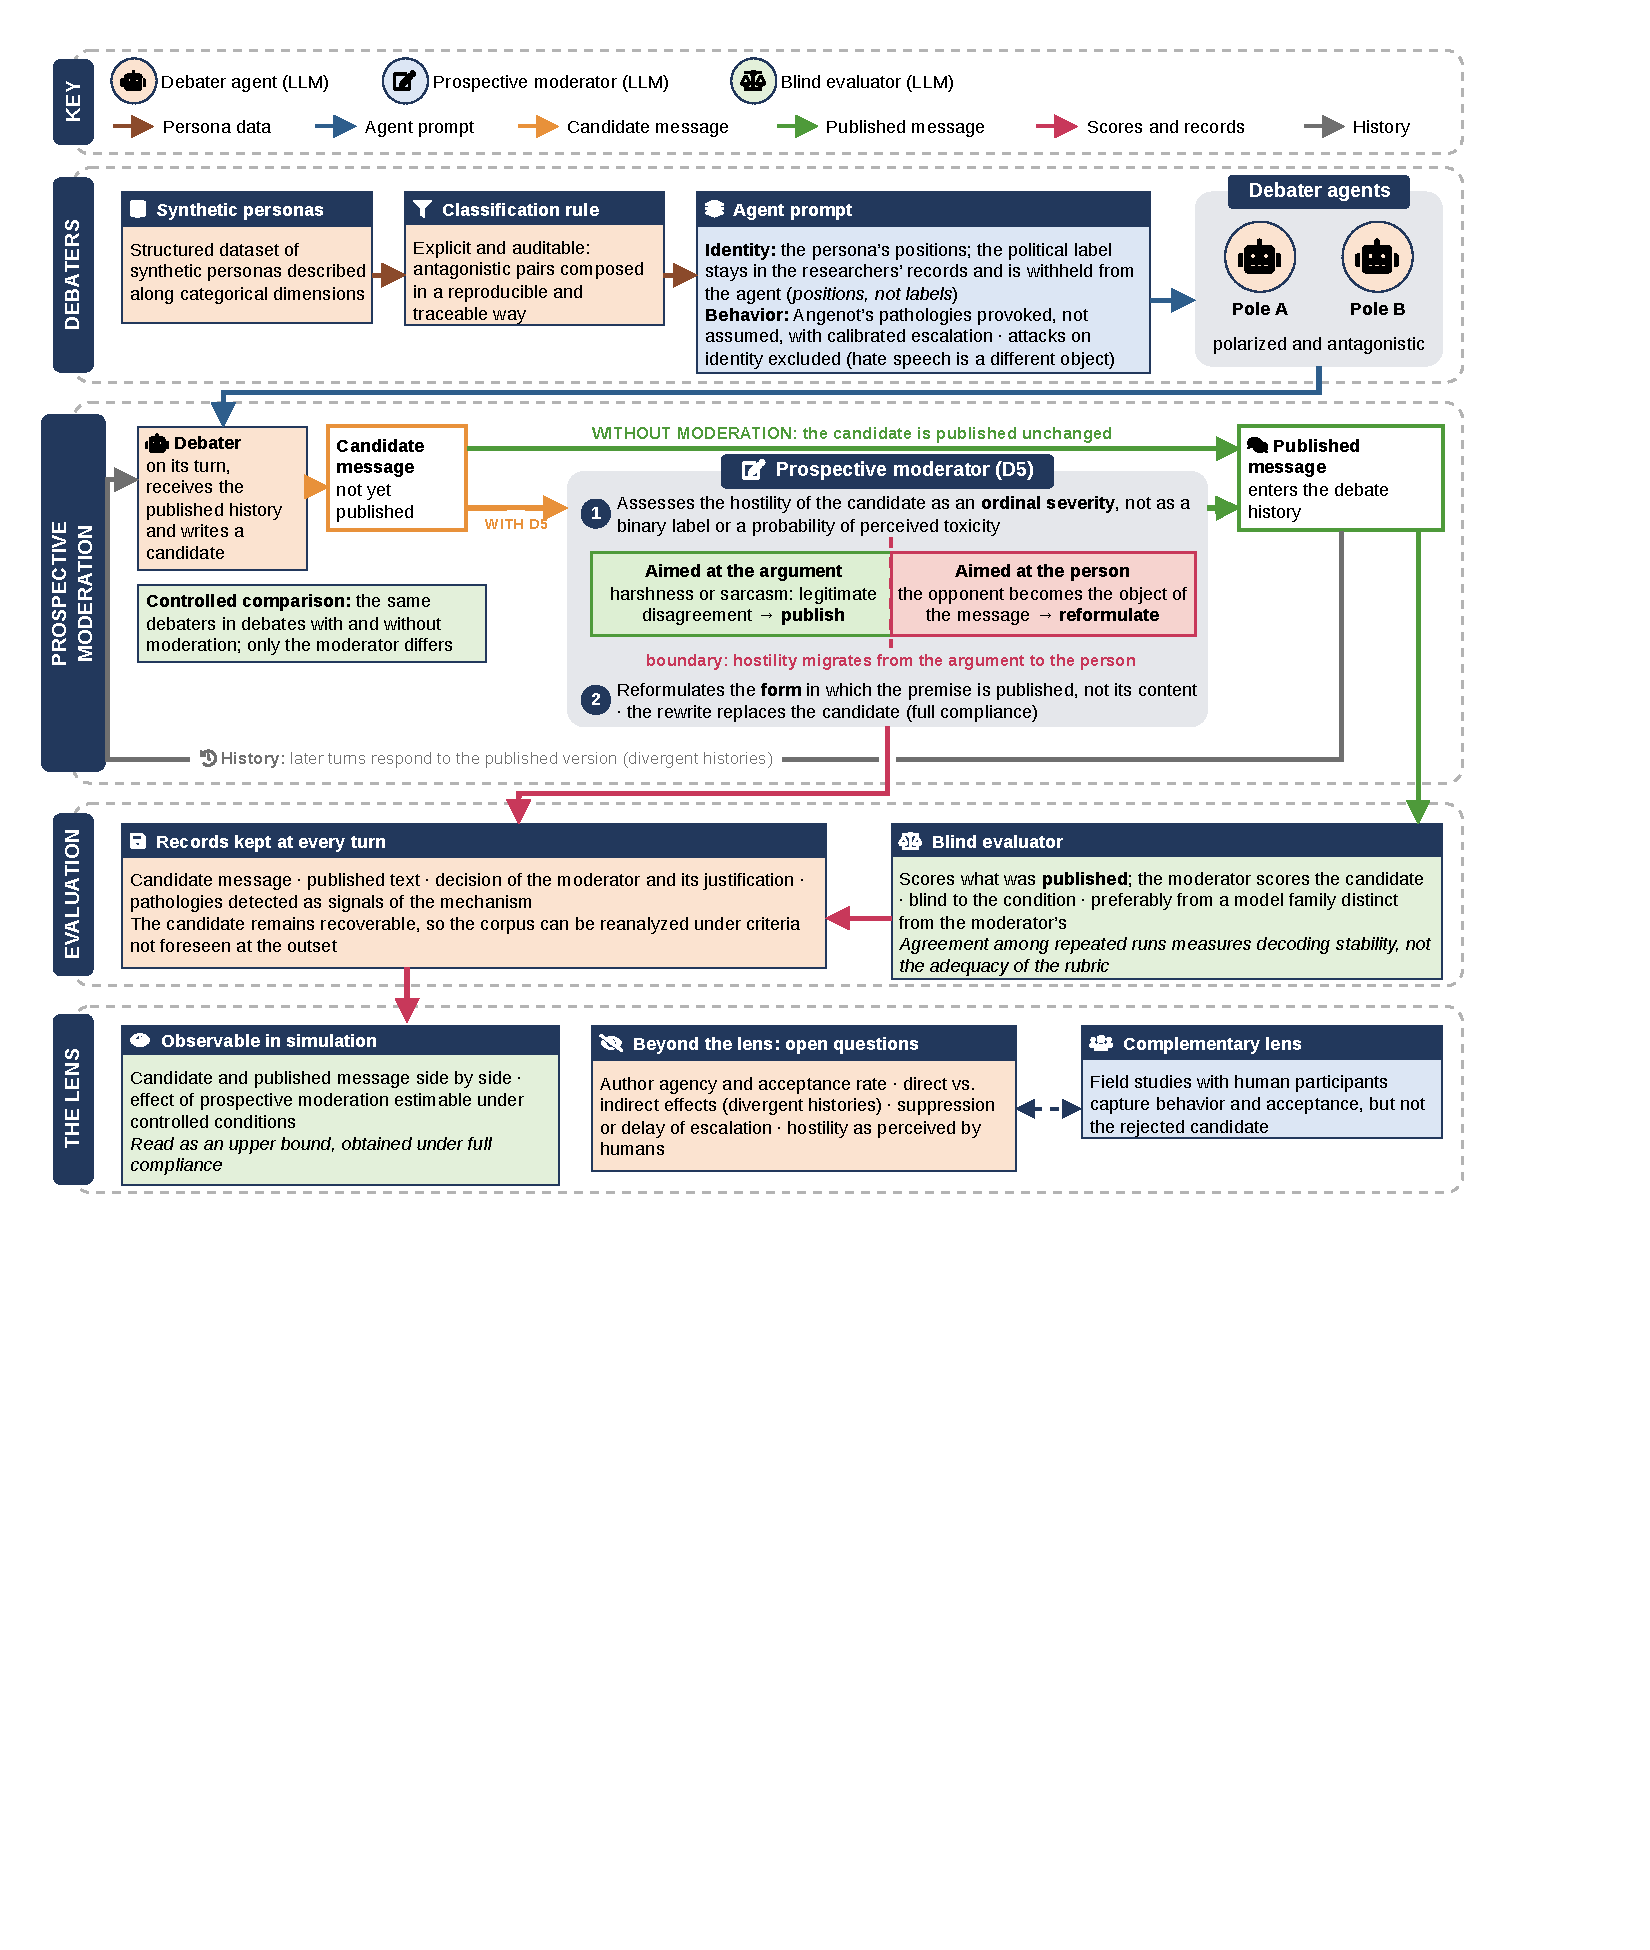
\includegraphics[width=0.92\textwidth]{figures/pipeline_ismsit.pdf}
\caption{Conceptual pipeline of simulation with LLM agents as a lens on
prospective moderation. Arrow colors indicate the type of data exchanged
between stages; instruments, thresholds, and parameters are left to the
empirical report.}
\label{fig:pipeline}
\end{figure*}

\begin{table}[t]
\caption{What Each Lens Makes Observable}
\label{tab:lenses}
\centering
\renewcommand{\arraystretch}{1.25}
\begin{tabularx}{\columnwidth}{@{}>{\raggedright\arraybackslash}p{2.7cm}>{\raggedright\arraybackslash}X>{\raggedright\arraybackslash}X@{}}
\toprule
 & \textbf{Field studies}~\cite{argyle2023leveraging,katsaros2022reconsidering} & \textbf{LLM-agent simulation} \\
\midrule
Candidate message before the intervention & Unavailable once withdrawn or rewritten & Recorded at every turn \\
Effect of the reformulation itself & Not isolable & Estimable under controlled conditions \\
Author's decision (acceptance rate) & Central outcome & Not observable \\
Reactions of real users & Captured & Not captured \\
\bottomrule
\end{tabularx}
\end{table}

\subsection{Conditions for an Informative Simulation}\label{sec:conditions}

A simulation of this kind is informative only under certain conditions, which
follow from the arguments above.

\begin{itemize}
\item \textbf{Conflict must be provoked, not assumed.} Given the tendency of
LLM agents toward consensus and politeness~\cite{chuang2023simulating}, a
simulation left to itself would produce debates with little to moderate.
Angenot's categories therefore play a double role: they configure the
behavior of the debaters, with explicitly calibrated escalation, so that the
debate is genuinely unproductive; and they serve as qualitative signals of the
mechanism at work. A boundary must nonetheless be kept: attacks on conduct or
character belong to the unproductive debate under study, whereas attacks on
identity, religion, nationality, or disability belong to hate speech, which is
a different object.
\item \textbf{Polarization should come from positions, not labels.} When
antagonistic personas are derived from structured
datasets~\cite{li2026matraix}, handing the agent its political label would
lead the model to attend to the label rather than to the persona's positions,
with two risks: importing implicit attributes that were never declared, and
flattening the variation within each pole by pulling distinct personas toward
a common prototype. The label can remain in the researchers' records while
being withheld from the agent.
\item \textbf{The instrument that moderates must not be the one that
evaluates.} The moderator scores the candidate message before publication;
the evaluator scores what was published. Under moderation, these messages
differ whenever an intervention occurred, and conflating them would compare a
message with its own substitute. An evaluator blind to the condition,
preferably built on a model family distinct from that of the moderator,
prevents the same system from judging its own intervention.
\item \textbf{The candidate must remain recoverable.} Since the difference
between the candidate and the published message is the very object of
inquiry, both must be preserved at every turn, together with the decision of
the moderator and its justification. Such records make the corpus
reanalyzable under criteria not foreseen at the outset.
\end{itemize}

\section{Open Questions}\label{sec:open}

The limits of the lens are not accidental: each follows from a choice that
makes observation possible. Three questions remain open and are offered for
discussion.

\textbf{Author agency and compliance.} In a simulation, the reformulation can
replace the candidate without an acceptance step. Delegating that decision to
an LLM agent would lack an empirical anchor and would inherit the consensus
and politeness bias of such agents~\cite{chuang2023simulating}, most likely
yielding artificially high acceptance. Any effect estimated in this way is
therefore an upper bound obtained under full compliance, and the acceptance
rate, which is the central variable in studies with
humans~\cite{argyle2023leveraging,katsaros2022reconsidering}, is not
observable in such a design. Reintroducing author agency, whether by
parameterizing the decision with empirical rates from the
literature~\cite{katsaros2022reconsidering} or by placing humans in the loop,
is what would turn an upper bound into an estimate of the expected effect.

\textbf{Divergent histories.} Once a message is reformulated, a moderated
debate and its unmoderated counterpart no longer share the same history,
since later turns respond to the moderated version. Any difference between
them combines the direct effect of the rewriting with the indirect
de-escalation of an interlocutor who receives a milder text. For platform
design, this combined effect of the presence of the moderator in the system
is probably the relevant quantity, since a real deployment would produce both
at once; for understanding the mechanism, however, the distinction matters,
and separating the two remains an open problem.


\textbf{Validity of the lens.} Simulated personas are caricatural by
construction: they serve to provoke the pathologies in a controlled
environment, not to represent real voters. Synthetic hostility also tends to
be cleaner than real hostility, lacking the obscure irony, the rumor, and the
typographic noise of authentic online discourse. Until inter-annotator
agreement is established~\cite{krippendorff2011computing} and the cultural
dependence of perceived
hostility~\cite{papacharissi2004democracy,rossini2022beyond} is addressed, the
scores produced by agents instructed with a rubric remain instrumental
classifications rather than validated measures of hostility as perceived by
humans.

\section{Conclusion}\label{sec:conclusion}

This paper argued that prospective moderation, the regulation of conduct in
the interval between the production and the publication of a message, faces
an evaluation problem that is conceptual before it is empirical: its effect
lies in a message that, on a real platform, ceases to exist as observable
data. Building on Angenot's dialogue of the deaf, it argued that such
moderation should act on the form of an exchange rather than on its content;
building on the incivility literature, it argued that the threshold for
intervention lies where hostility migrates from the argument to the person,
and that hostility is better treated as an ordinal severity than as a binary
label or a probability of perceived toxicity. Simulation with LLM agents was
then discussed as a lens that trades behavioral realism for full
observability, complementary to field studies with human participants.

None of the limits discussed is accidental, and each points to a line of
work: the validation of the instruments against human judgment, the
reintroduction of author agency, and the separation between the direct and
indirect effects of moderation. The broader question left open for
discussion is whether the effectiveness of mitigating unproductive debates
depends less on the potency of each isolated mechanism than on the
composition among them. Examining that composition is the next step of the
research agenda from which these positions derive.

\bibliographystyle{IEEEtran}
\bibliography{references}

\end{document}
